\subsubsection{User Interfaces}

This section presents the user interfaces of the web platform. For students and companies, examples are provided to illustrate how the interfaces could appear on desktop and mobile applications. These examples include the login page, sign-up pages tailored for students and companies, and the main pages specific to each user type.

The student interface focuses on features such as searching for internships and applying to opportunities. The company interface highlights functionalities like creating internships, reviewing existing ones, and displaying important information about each internship.


\bigskip

\begin{figure}[ht]
    \centering
    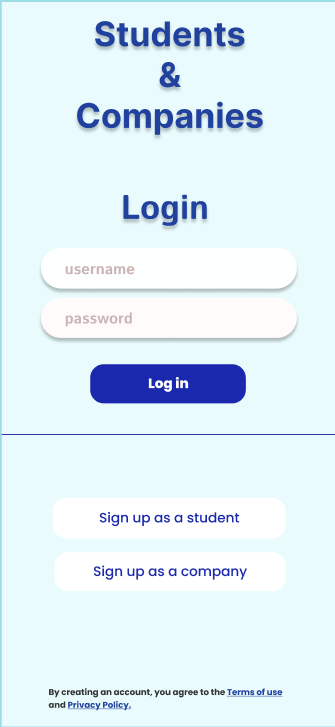
\includegraphics[width=0.45\textwidth]{RASD-Latex/assets/UI images/login_phone.png}
    \caption{Log in form on mobile application}
    \label{fig:image1}
\end{figure}


\begin{figure}[ht]
    \centering
    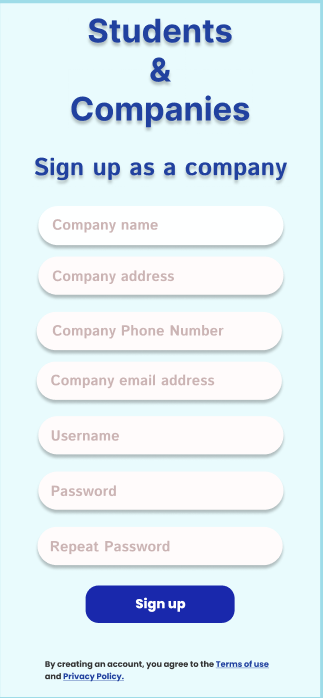
\includegraphics[width=0.45\textwidth]{RASD-Latex/assets/UI images/signup_company_phone.png}
    \caption{Sign up for companies on mobile application}
    \label{fig:image1}
\end{figure}



\begin{figure}[ht]
    \centering
    \begin{minipage}{0.45\textwidth}
        \centering
        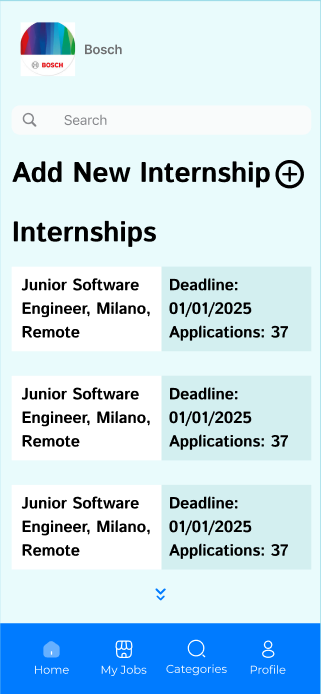
\includegraphics[width=\textwidth]{RASD-Latex/assets/UI images/mainpage_company_phone.png}
        \caption{Main page for companies on mobile application}
        \label{fig:image1}
    \end{minipage}
    \hspace{0.05\textwidth}  % Optional space between the images
    \begin{minipage}{0.45\textwidth}
        \centering
        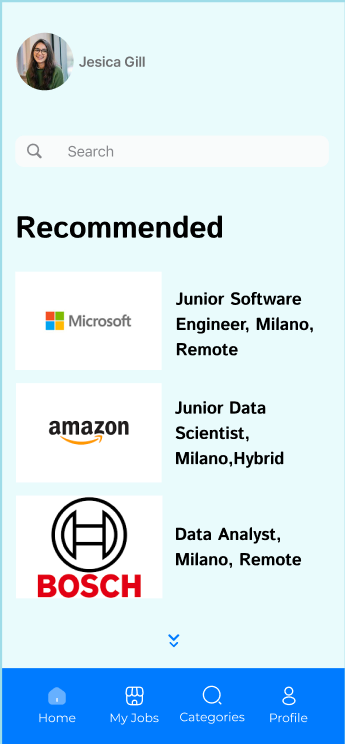
\includegraphics[width=\textwidth]{RASD-Latex/assets/UI images/mainpage_student_phone.png}
        \caption{Main page for students on mobile application}
        \label{fig:image2}
    \end{minipage}
\end{figure}

\clearpage

\begin{figure}[h!]
    \centering
    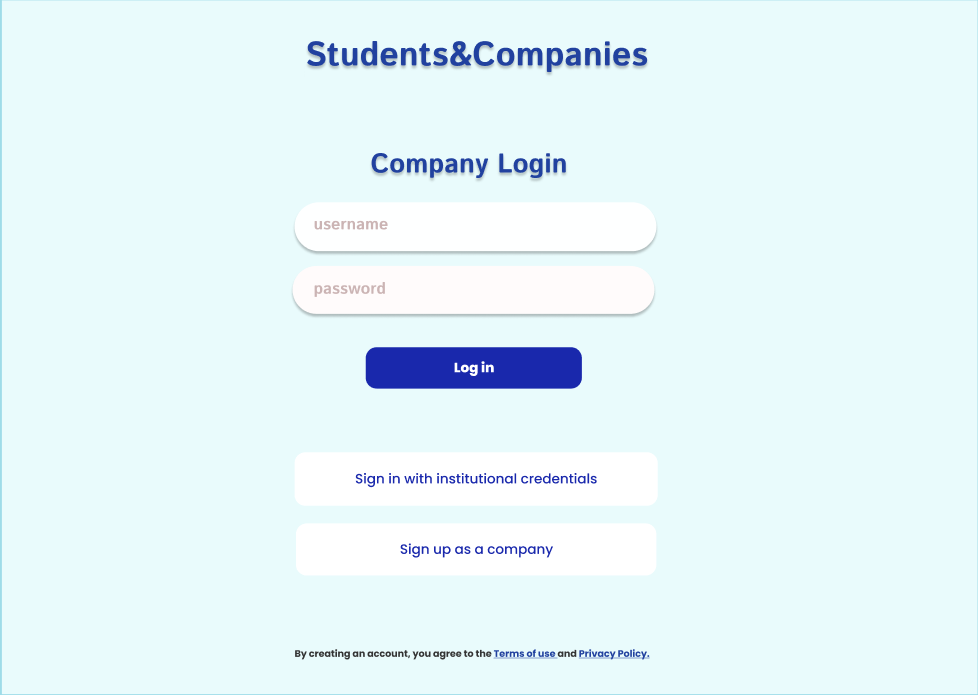
\includegraphics[width=0.8\textwidth]{RASD-Latex/assets/UI images/login_desktop.png}
    \caption{Log in form on desktop application}
    \label{fig:image1}
\end{figure}


\begin{figure}[h!]
    \centering
    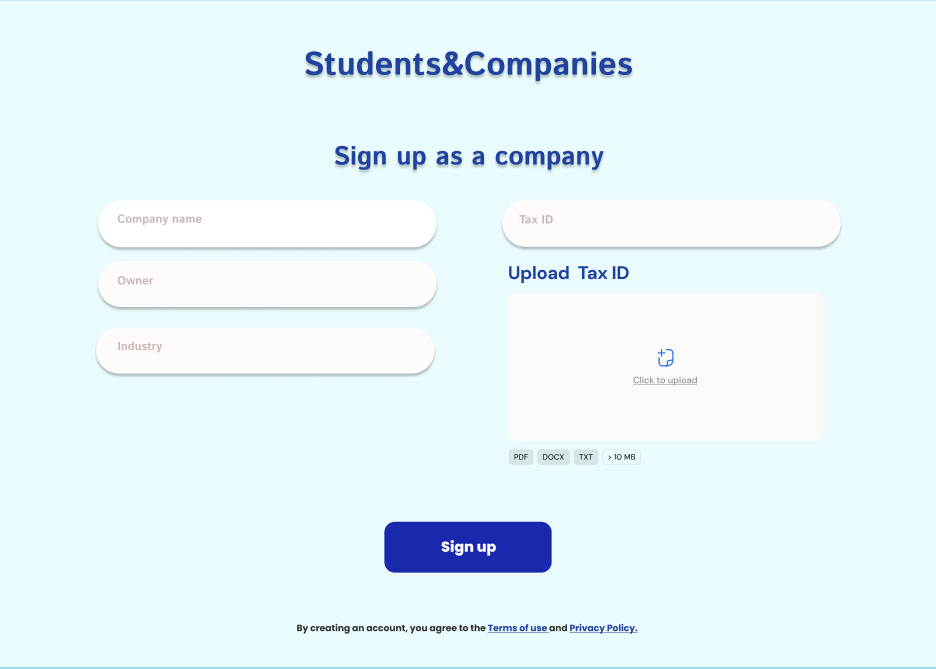
\includegraphics[width=0.8\textwidth]{RASD-Latex/assets/UI images/signup_company_desktop.png}
    \caption{Sign up for companies on desktop application}
    \label{fig:image1}
\end{figure}


\begin{figure}[ht]
    \centering
    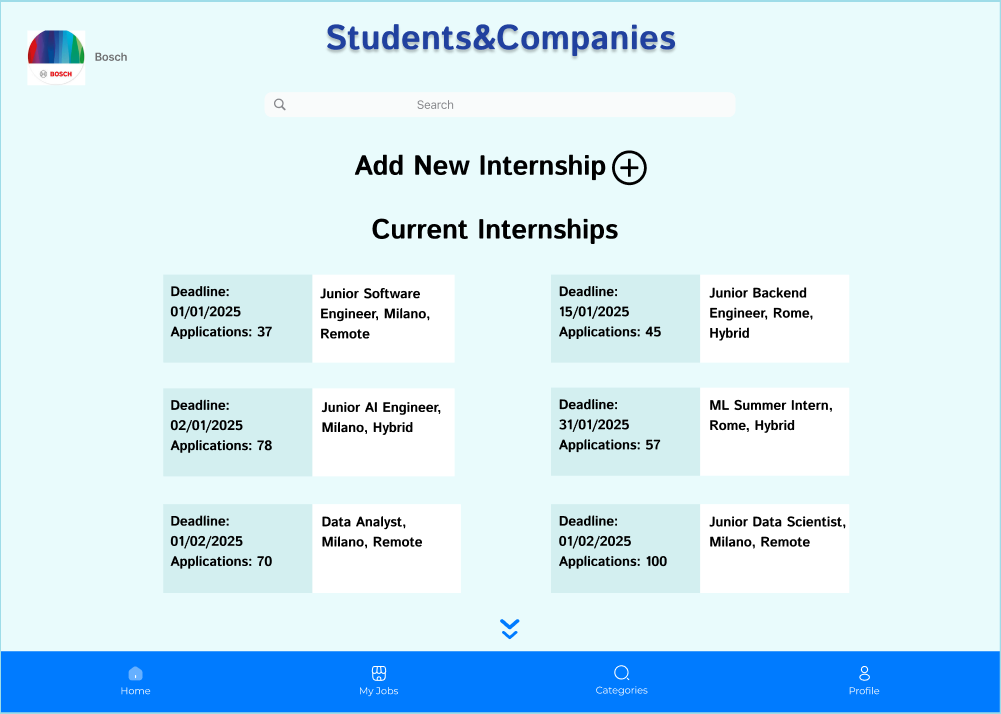
\includegraphics[width=0.8\textwidth]{RASD-Latex/assets/UI images/mainpage_company_desktop.png}
    \caption{Main page for companies on desktop application}
    \label{fig:image1}
\end{figure}


\begin{figure}[ht]
    \centering
    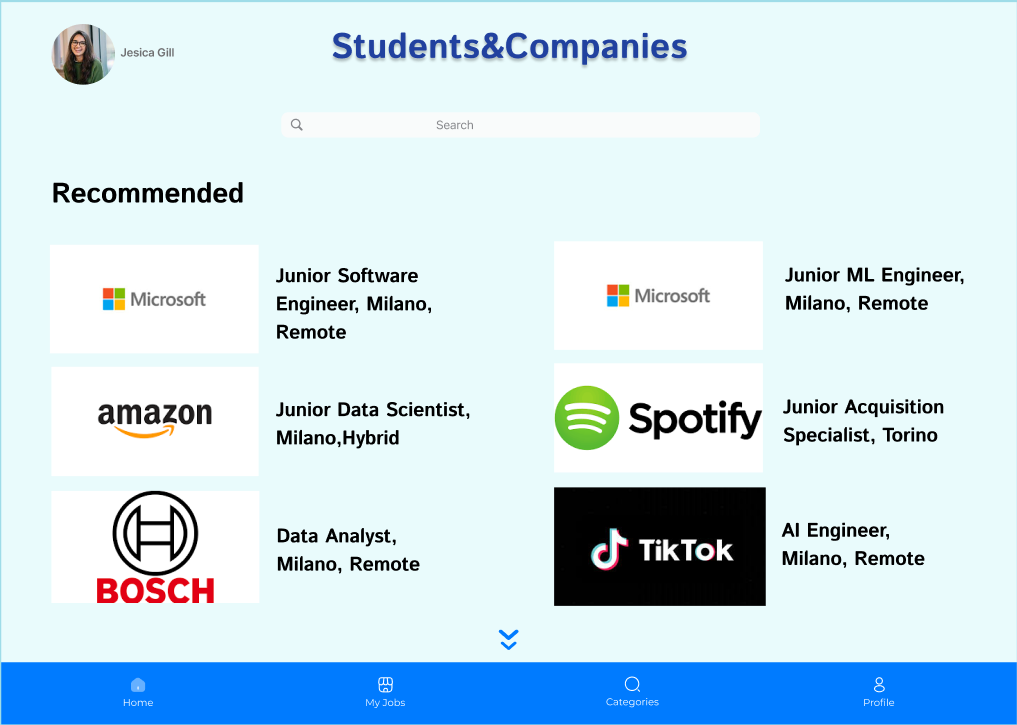
\includegraphics[width=0.8\textwidth]{RASD-Latex/assets/UI images/mainpage_student_desktop.png}
    \caption{Main page for students on desktop application}
    \label{fig:image2}
\end{figure}




\clearpage
\subsubsection{Hardware Interfaces}
While the platform is primarily a web application, specific hardware requirements exist to fully utilize all available features.

The minimum requirement for accessing and using the platform is a keyboard and a device that supports a modern browser compliant with HTML5 standards, as the user interface will comply with keyboard accessibility standards outlined in the Web Content Accessibility Guidelines (WCAG) 2.1.

Although not mandatory, using a pointing device is encouraged for efficiency. No specific pointer device is required for PCs or mobile devices, as the HID protocol and touchscreens are widely supported.

% Ovo je moj tekst za MFA od kojeg sam odustao na kraju
% As the platform will support multi-factor authentication (MFA), users are encouraged (but not required) to possess an external iOS- or Android-based mobile device for this feature. MFA will be supported through an authenticator app and/or passkeys.

% Passkeys can be configured using in-built fingerprint readers and/or face-ID scanners on mobile devices. Therefore, users will need a fingerprint- or face-ID-enabled mobile device to configure and use passkeys.

% Lastly, the platform will allow users to register a FIDO2/WebAuthn-compliant hardware authenticator (e.g., from Yubico). To use this feature, users must possess the hardware authenticator as well as either an NFC-enabled mobile device or an HID-compliant USB port on any platform.

A summary of the described hardware interfaces is provided below.

\paragraph{Mandatory Hardware Interface Requirements (MHIR)}
\begin{itemize}
    \item \textbf{MHIR1.} An HID-compliant keyboard
\end{itemize}

\paragraph{Recommended Hardware Interface Requirements (RHIR)}
\begin{itemize}
    \item \textbf{RHIR1.} An HID-compliant pointer device
    % \item \textbf{RHIR2.} A fingerprint- or face-ID-enabled mobile device
\end{itemize}

% \paragraph{Optional Hardware Interface Requirements (OHIR)}
% \begin{itemize}
%     \item \textbf{OHIR1.} A FIDO2/WebAuthn-compliant hardware authenticator
%     \item \textbf{OHIR2.} An NFC-enabled smartphone
%     \item \textbf{OHIR3.} A device with an HID-compliant USB port
% \end{itemize}


\subsubsection{Software Interfaces}

As noted, in order for the application to be accessed, it must be done through a modern, HTML5-compliant browser, regardless of the operating system or browser type. 

The platform will be fully hosted on Amazon Web Services (AWS), so access to specific AWS APIs (e.g., AWS S3, AWS Lambda) and their associated endpoints will be required for its proper functionality.
% Additionally, the MFA feature will utilize the Time-Based One-Time Password (TOTP) API.

Furthermore, as part of the platform's Artificial Intelligence (AI) integration to enhance user profiles, the OpenAI ChatGPT API will be employed. 
For legacy system compatibility (e.g., older authentication methods), additional APIs will also be included to ensure backward compatibility.

% The platform may also support additional MFA methods, such as SMS-based codes or hardware tokens, to accommodate different user preferences.

A summary of the described software interfaces is provided below.

\paragraph{Mandatory Software Interface Requirements (MSIR)}
\begin{itemize}
    \item \textbf{MSIR1.} A modern, Web2-compliant browser
    \item \textbf{MSIR2.} AWS API and subsequent endpoints (e.g., AWS S3, AWS Lambda)
    \item \textbf{MSIR3.} OpenAI ChatGPT API
    \item \textbf{MSIR4.} WebPurify for text checking.
    \item \textbf{MSIR4.} API for institutional account linking and data processing

    % \item \textbf{MSIR4.} WebAuthn for FIDO2 authentication
    % \item \textbf{MSIR5.} U2F (Universal 2nd Factor), a legacy FIDO protocol for second-factor authentication
    % \item \textbf{MSIR6.} TOTP API for generating one-time passwords
    % \item \textbf{MSIR7.} Twilio or Nexmo API for sending SMS-based one-time passcodes
    % \item \textbf{MSIR8.} OATH OTP algorithm or FIDO2/WebAuthn for hardware token-based authentication
\end{itemize}




\subsubsection{Communication Interfaces}
The communication between the web application and backend systems, as well as external services, will primarily use the HTTPS protocol. The application will interact with the provided endpoints via RESTful APIs for all CRUD operations, where all data exchanged will be encrypted in transit using TLS (Transport Layer Security) and stored securely in the system's database using industry-standard encryption methods. Moreover, WebSocket connections will utilized primarily for push-notifications. Lastly, as there will most likely be other system crucial third party services, their provided API gateways will be utilized within the application.
